\documentclass[border=15pt]{standalone}
\usepackage{amsmath,amssymb,mathtools}
\usepackage{tikz}
\usepackage{pgfplots}
\usepackage{pgf}
\begin{document}
	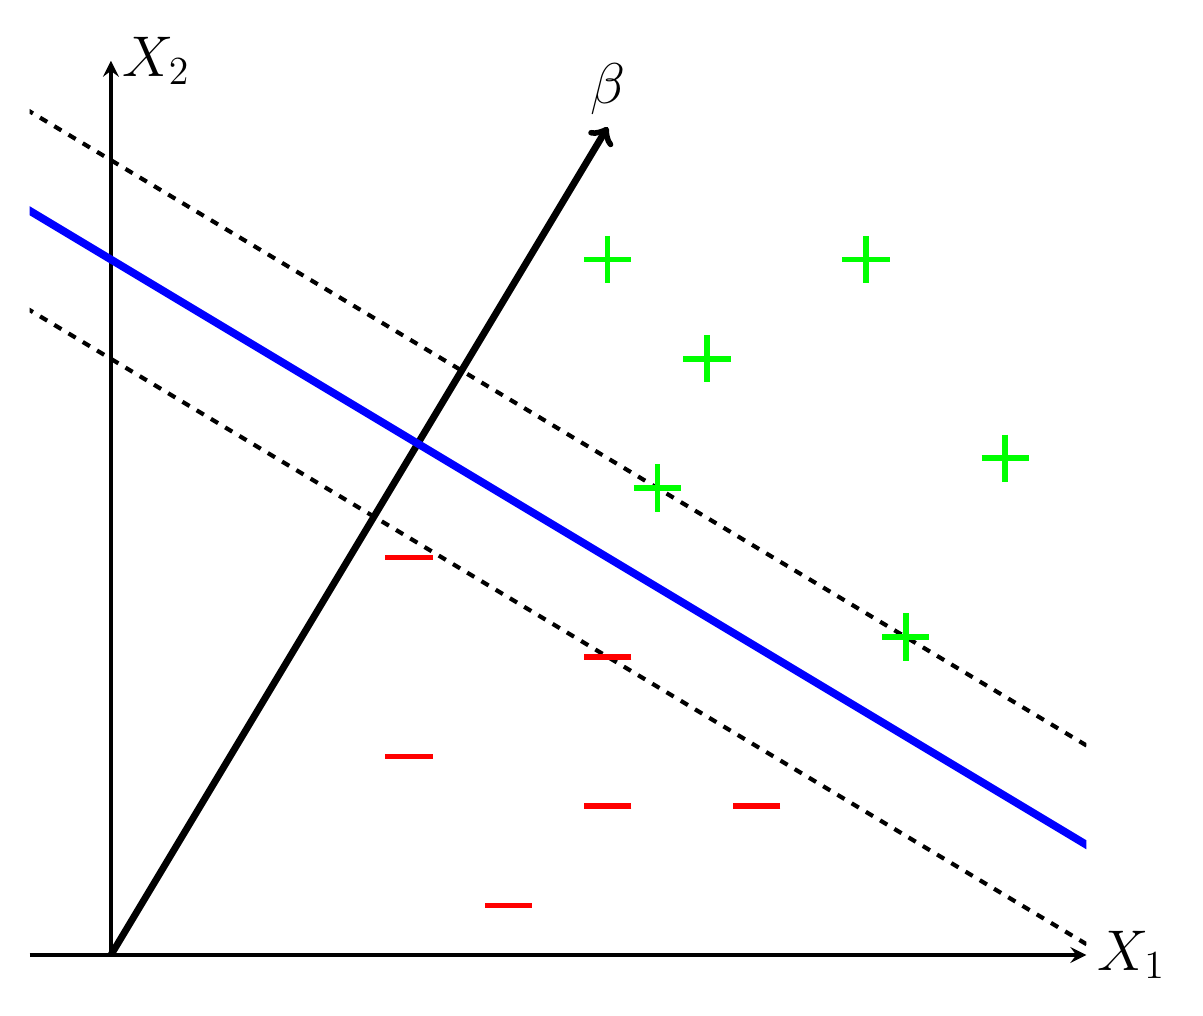
\begin{tikzpicture}
		\begin{axis}[
			xmin=0,
			xmax=9,
			ymin=0,
			ymax=9,
			axis equal,
			width=15cm,
			axis x line=center,
			axis y line=center,
			xmajorticks=false,
			ymajorticks=false,
			ylabel style={right,font=\huge},
			ylabel=$X_2$,
			xlabel style={above,right,font=\huge},
			xlabel=$X_1$,
			line width=1.5pt
			]
			%\addplot[no markers, domain=-1:11]{(5/3)*x};
			
			\draw[->,line width=2.5pt] (axis cs:0,0)--(axis cs:5,8.333) node[above,pos=1,font=\huge]{$\beta$};
			\addplot[only marks, mark=+,draw=green,mark size=0.3cm,line width= 2pt]coordinates {(8,3.2)
			(8,3.2) (5,7) (6,6) (9,5) (7.6,7) (5.5,4.7)};
			\addplot[only marks, mark=-,draw=red,mark size=0.3cm,line width=2pt]coordinates {(3,4)
			(5,3) (3,2) (5,1.5) (4,0.5) (6.5,1.5)};
			\addplot[no markers,domain=-1:11,thick,blue,line width=2.8pt]{-0.6*x+7};
			\addplot[no markers, domain=-1:11,dashed,line width=1.5pt]{-0.6*x+8};
			\addplot[no markers, domain=-1:11,dashed,line width=1.5pt]{-0.6*x+6};
		\end{axis}
	\end{tikzpicture}
\end{document}